%%%%%%%%%%%%%%%%%%%%%%%%%%%%%%%%%%%%%%%%%
% FRI Data Science_report LaTeX Template
% Version 1.0 (28/1/2020)
%
% Jure Demšar (jure.demsar@fri.uni-lj.si)
%
% Based on MicromouseSymp article template by:
% Mathias Legrand (legrand.mathias@gmail.com)
% With extensive modifications by:
% Antonio Valente (antonio.luis.valente@gmail.com)
%
% License:
% CC BY-NC-SA 3.0 (http://creativecommons.org/licenses/by-nc-sa/3.0/)
%
%%%%%%%%%%%%%%%%%%%%%%%%%%%%%%%%%%%%%%%%%


%----------------------------------------------------------------------------------------
%	PACKAGES AND OTHER DOCUMENT CONFIGURATIONS
%----------------------------------------------------------------------------------------
\documentclass[fleqn,moreauthors,10pt]{ds_report}
\usepackage[english]{babel}

\graphicspath{{fig/}}




%----------------------------------------------------------------------------------------
%	ARTICLE INFORMATION
%----------------------------------------------------------------------------------------

% Header
\JournalInfo{Machine Learning for Data Science 1, 2025-2026}

% Interim or final report
%\Archive{Interim report}
\Archive{Homework 2 Report}

% Article title
\PaperTitle{Model Evaluation and Error Analysis}

% Authors and their info
\Authors{Tjaš Ajdovec}
\affiliation{\textit{ta5946@fri.uni-lj.si}}

% Multiple authors
%\Authors{John Doe\textsuperscript{1}, Jane Doe\textsuperscript{2}, and Mike Smith\textsuperscript{3}}
%\affiliation{\textsuperscript{1}\textit{john.doe@fri.uni-lj.si}}
%\affiliation{\textsuperscript{1}\textit{jane.doe@fri.uni-lj.si}}
%\affiliation{\textsuperscript{1}\textit{mike.smith@fri.uni-lj.si}}

%----------------------------------------------------------------------------------------

\makeatletter
\renewcommand{\@maketitle}{%
\twocolumn[{%
\thispagestyle{empty}%
{
\includegraphics[height=2cm]{logo}}
\vskip-74pt%
{\raggedleft\small\sffamily\bfseries\@JournalInfo\\\@Archive\par}%
\vskip64pt%
{\raggedright\color{color1}\fontfamily{cmss}\fontseries{bc}\fontshape{n}\fontsize{20}{25}\selectfont \@PaperTitle\par}%
\vskip10pt%
{\raggedright\color{color1}\sffamily\fontsize{12}{16}\selectfont  \@Authors\par}%
\vskip8pt%
\begingroup%
\raggedright\sffamily\small%
\footnotesize\@affiliation\par%
\endgroup%
\vskip10pt%
}]%
}
\makeatother

\begin{document}

% Makes all text pages the same height
\flushbottom

% Print the title and abstract box
\maketitle

% Removes page numbering from the first page
\thispagestyle{empty}

%----------------------------------------------------------------------------------------
%	ARTICLE CONTENTS
%----------------------------------------------------------------------------------------

\section*{Introduction}
    In this homework, we implemented a model evaluator Python class. This takes in a dataset, a scikit-learn compatible model, and the hyperparameter to optimize. It uses $k$-fold cross-validation (CV) to evaluate the model and either minimizes training fold loss or performs nested CV for parameter selection.

    We evaluated three standard models on the provided basketball dataset of shots. We analyzed the classification error rate for specific feature values and estimated accuracy on a real-world distribution with different relative class frequencies.

%------------------------------------------------

\section*{Part 1: Nested Cross-Validation}

We first deduplicated and shuffled the dataset. Our objective was to predict the \textit{ShotType} based on other fields. We compared \textit{DummyClassifier}, which always predicts the relative class frequency, \textit{LogisticRegression} (LR) with tunable parameter $C$, and \textit{KNeighborsClassifier} (KNN) with $n\_neighbors$. During training, we \textbf{minimized log-loss} but also reported classification accuracy:

\begin{equation}
L = - \frac{1}{n} \sum_{i=1}^{n} \sum_{j=1}^{C} y_{\text{true},ij} \log\left(y_{\text{prob},ij}\right)
\end{equation}

\begin{table}[h!]
    \centering
    \begin{tabular}{l c c}
        \toprule
        \textbf{Model} & \textbf{Accuracy} & \textbf{Log-Loss} \\
        \midrule
        Relative frequency & $0.609 \pm 0.015$ & $1.170 \pm 0.032$ \\
        LR + train CV      & $0.731 \pm 0.016$ & $0.680 \pm 0.035$ \\
        \textbf{LR + nested CV}     & $\mathbf{0.731 \pm 0.016}$ & $\mathbf{0.680 \pm 0.035}$ \\
        KNN + train CV     & $0.683 \pm 0.015$ & $6.359 \pm 0.481$ \\
        \textbf{KNN + nested CV}    & $\mathbf{0.695 \pm 0.018}$ & $\mathbf{1.000 \pm 0.093}$ \\
        \bottomrule
    \end{tabular}
    \vspace{0.5em}
    \caption{Estimated classification accuracies, log-losses, and standard errors for all evaluated models.}
    \label{tab1}
\end{table}

We compared two model evaluation approaches. Both use \textbf{outer k-fold CV} for estimating the model performance. However, for each outer validation:

\begin{enumerate}
    \item Optimizes the parameters \textbf{directly on the training fold}, which is a biased tuning strategy that tends to overfit and leads to worse model results.
    \item Splits the outer training fold into \textbf{inner k-folds and conducts another CV}, where it tracks the average log-loss for each parameter configuration. This way of tuning is computationally more expensive but results in a model with better generalization.
\end{enumerate}

We used $k=5$ folds both for inner and outer CV. The results for different models and evaluation approaches are presented in Table~\ref{tab1}. We observed that all models \textbf{outperformed the baseline classification accuracy of 61\%}. LR remained stable for both parameter tuning strategies. \textbf{KNN} proved to be more \textbf{sensitive to overfitting}, as the direct training optimization CV resulted in a limited $n\_neighbors=3$ and lower validation accuracy and log-loss. Besides that:
\begin{itemize}
    \item \textbf{Removing duplicate instances} lowered the overall accuracy by around 0.5\%, which was expected.
    \item \textbf{Increasing the outer k} to 10 slightly increased the performance as well as the standard error. This is likely a consequence of more training data and fewer validation instances per fold.
\end{itemize}

We collected target class predictions and probabilities from each validation fold and analyzed them in Part 2.

%------------------------------------------------

\section*{Part 2: Error Analysis}

\begin{table}[h!]
    \centering
    \begin{tabular}{l c c c}
        \toprule
        \textbf{Competition} & \textbf{Sample Freq} & \textbf{Real Freq} & \textbf{Difference} \\
        \midrule
        \textbf{NBA}  & $\mathbf{0.248}$ & $\mathbf{0.600}$ & $\mathbf{-0.352}$ \\
        EURO & $0.271$ & $0.100$ & $+0.171$ \\
        SLO1 & $0.232$ & $0.100$ & $+0.132$ \\
        U14  & $0.147$ & $0.100$ & $+0.047$ \\
        U16  & $0.102$ & $0.100$ & $+0.002$ \\
        \bottomrule
    \end{tabular}
    \vspace{0.5em}
    \caption{Comparison of the sample dataset and real-world distribution of shots by competition.}
    \label{tab2}
\end{table}

\begin{figure*}[h!]
    \centering
	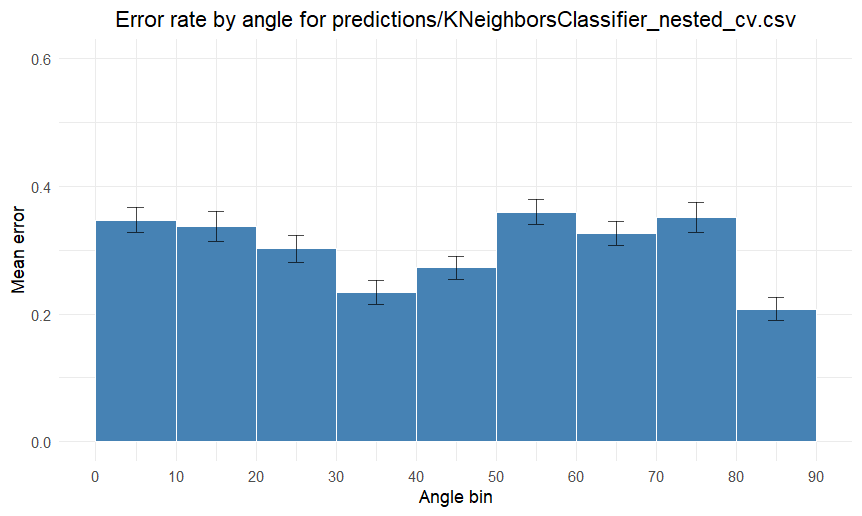
\includegraphics[width=0.75\linewidth]{fig/knn_error_by_angle.png}
    \caption{Estimated misclassification rates and standard errors for shot angles grouped in 10° intervals.}
	\label{fig1}
\end{figure*}

This part was done entirely in R. First, we checked how the estimated classification error depends on the shot \textit{Angle}. We \textbf{grouped angles in 10° bins} and plotted the associated misclassification rates, as shown in Figure~\ref{fig1}. We noticed that the type of \textbf{shots from the corner} (80 to 90 degrees) and the \textbf{elbow-wing} (30 to 50 degrees) were \textbf{easier to determine}.
This was consistent across all inspected models.

Secondly, we were given the real-world basketball game \textit{Competition} distribution. This was different from our dataset, as seen in Table~\ref{tab2}. To estimate real-world performance, we \textbf{calculated the accuracy for each competition} and multiplied it by the provided relative frequencies. Because our models were already better at predicting NBA games, the \textbf{estimated real-world accuracy was about 2\% higher}.

\begin{table}[h!]
    \centering
    \begin{tabular}{l c c c}
        \toprule
        \textbf{Model} & \textbf{Sample Acc} & \textbf{Real Acc} & \textbf{Change} \\
        \midrule
        Relative frequency      & $0.609$ & $0.632$ & $+0.023$ \\
        \textbf{LR + nested CV} & $\mathbf{0.731}$ & $\mathbf{0.752}$ & $\mathbf{+0.021}$ \\
        KNN + nested CV & $0.695$ & $0.710$ & $+0.015$ \\
        \bottomrule
    \end{tabular}
    \vspace{0.5em}
    \caption{Comparison of the estimated sample dataset and real-world accuracy of shot type prediction.}
    \label{tab3}
\end{table}

\section*{Part 3: CV for Spatial Data}

Regular CV for model performance estimation on spatially dependent data can lead to an \textbf{optimistic bias when moving to new areas}. The article \cite{mahoney2023assessingperformancespatialcrossvalidation} compares different CV approaches for spatial data and evaluates them on 100 simulated landscapes. Their methods are implemented in the \textit{spatialsample} R package. In this section, we denote a single training fold as $D_{in}$ and a validation fold as $D_{out}$.

\begin{enumerate}
    \item \textbf{Resubstitution} uses all instances in both $D_{in}$ and $D_{out}$, which results in a strongly optimistic estimate.
    \item \textbf{Random V-fold} CV also tends to be optimistic when dealing with hidden dependencies, such as spatial data.
    \item \textbf{Blocked} CV divides the instances using a parametrized grid and $D_{out}$ buffers. However, spatial structures are rarely grid-like.
    \item \textbf{Clustered} CV captures the spatial structure by creating clusters and using them as folds. It is flexible in the choice of the distance metric but may be non-deterministic.
    \item Buffered Leave-One-Observation-Out (\textbf{BLO3}) CV treats each instance as a separate $D_{out}$ and uses a fixed distance exclusion buffer. Small validation folds can lead to unstable estimates. 
    \item Leave-One-Disc-Out (\textbf{LODO}) CV works in a similar way but uses both inclusion and exclusion buffers. It is relatively robust to parameter choices and can include the same instance in multiple $D_{out}$ sets.
    \item Nearest Neighbor Distance Matching (\textbf{NNDM}) tries to match the distributions of distances between training and validation points $G_{pp}$ with the expected distances between dataset (calibration) and target points $G_{cp}$. It requires defining the target prediction area.
\end{enumerate}

In their experiments and related work, Clustered and LODO produced the most realistic model performance estimates. This was likely due to correctly capturing the spatial dependencies in the data.

\bibliographystyle{unsrt}
\bibliography{report}

\end{document}
